% Aggregation methods — the two recombinable axes (grouping x representation),
% the optional post-steps, and the return path, in pipeline order.
%
% This is a CONCEPTUAL diagram, not a UML one: it is the companion to the
% how-aggregation-works overview and answers "what can I choose, and when does
% it apply", not "what modules exist". The building block view and the runtime
% view carry the UML notation.
%
% ── PRINT TARGET ──────────────────────────────────────────────────────────
% "AutoRecovery save of ETHOS.docx" is US Letter with 1 inch margins: text
% column 165.1 x 228.6 mm, and every figure in it is placed at the full 165 mm
% width (wp:extent cx="5943600" EMU). Word scales to that width, so the binding
% constraint is the ASPECT RATIO: at 165 mm wide the figure renders
% 165 * (h/w) mm tall and still needs room for a caption. Budget h/w <= 1.24.
% This file is 161 x 187 mm — aspect 1.16, so 191 mm tall in the document.
%
% ── WHICH ATTRIBUTE EACH MENU SETS ────────────────────────────────────────
% Every menu now carries a second title line naming the config attribute its
% chips are values FOR. Without it the diagram showed six representation names
% with no hint that they are what you assign to ClusterConfig.representation /
% SegmentConfig.representation (config.py:282, :426) rather than separate
% arguments of aggregate(). Same for ClusterConfig.method (:281) and
% ExtremeConfig.method (:488); the rescale chips really are plain aggregate()
% keyword arguments (api.py:35-36), and the subtitle says so.
%
% ── LEADERS: ORTHOGONAL, IN FIVE SEPARATE LANES ───────────────────────────
% The dotted leaders used to be straight diagonals fanning out of one point,
% which made it guesswork which stage fed which menu. They are now right-angle
% elbows, one per lane, in the 55..70 gutter:
%   x = 69  Normalize  (-33)  -> Scaling & weighting  (-25)
%   x = 66  GROUP      (-48)  -> Axis 1               (-60)
%   x = 63  REPRESENT  (-63)  -> Axis 2               (-100)
%   x = 60  Extremes   (-78)  -> Extreme periods      (-135)
%   x = 57  Rescale    (-93)  -> Rescale              (-160)
% The lane order is the load-bearing part and it is INVERTED with respect to
% the reading order: the leader that drops furthest gets the lane closest to
% the pipeline column. Assign them the other way round and every outgoing leg
% cuts through the lane of the leader below it — e.g. the extremes leg at
% y = -78 would cross Axis 2's lane, which spans -63..-100.
%
% Left column  = the pipeline, top to bottom. Required stages are solid blue;
%                optional steps are dashed amber. The dashes, not the colour,
%                carry the required/optional distinction, so the diagram still
%                reads in a greyscale print, and two swatches at the bottom say
%                so without spending a prose paragraph on it.
% Column x-ranges: left 3..55, gutter 55..70, right 70..162.
%
% Every stage box is kept to TWO lines of text so all ten fit an 11 mm box on a
% 15 mm pitch. Going to three lines costs 20 mm of height across the column,
% which is most of the caption's room.
%
% Non-ASCII must use LaTeX commands, not literal UTF-8: under T1 encoding a raw
% x-times sign, middle dot or em dash lands on the wrong glyph slot. Use
% $\times$, \textperiodcentered{} and ---.
%
% Regenerate:
%   tectonic aggregation_methods.tex
%   pdftocairo -svg aggregation_methods.pdf aggregation_methods.svg

\documentclass[10pt,border=1mm]{standalone}
\usepackage[T1]{fontenc}
\usepackage{lmodern}
\usepackage{tikz}
\usetikzlibrary{positioning,arrows.meta,fit,backgrounds}

\definecolor{fzjblue}{HTML}{023D6B}
\definecolor{fzjdark}{HTML}{012845}
\definecolor{tintblue}{HTML}{DCE9F2}
\definecolor{amber}{HTML}{A8681A}
\definecolor{ambertint}{HTML}{FBF1E4}
\definecolor{teal}{HTML}{21918C}
\definecolor{tealtint}{HTML}{EEF6F5}
\definecolor{greytext}{HTML}{3F4A55}

% Subtitle inside a menu title: a DECLARATION, not a one-argument macro, so it
% can be used as "{\msub ...}" inside the node text. It has to reset
% \normalfont as well as the size and colour, because the surrounding mtitle
% style is bold and coloured and a font switch alone would inherit both.
\newcommand{\msub}{\normalfont\scriptsize\color{greytext}}

\begin{document}
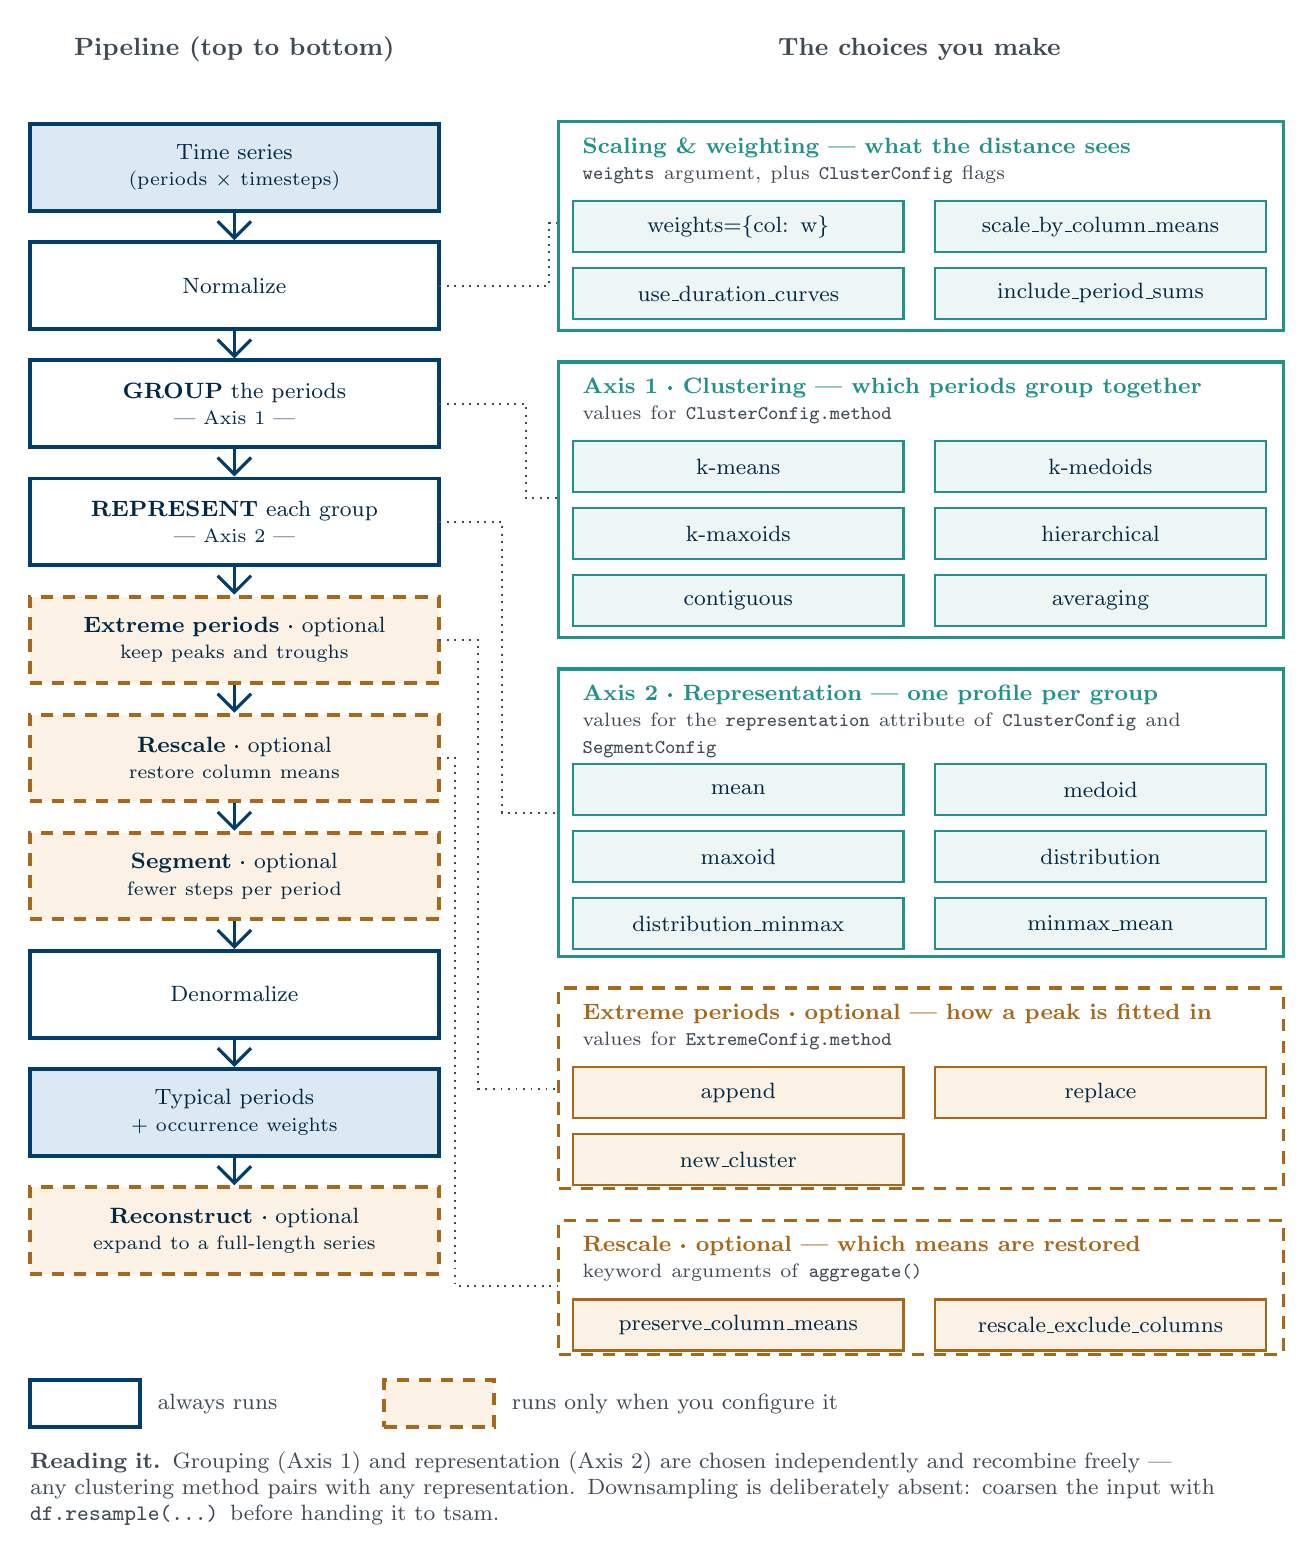
\begin{tikzpicture}[
  x=1mm, y=1mm,
  % required pipeline stage
  stage/.style={
    draw=fzjblue, line width=0.5mm, fill=white, text=fzjdark,
    minimum width=52mm, minimum height=11mm, text width=48mm,
    align=center, font=\footnotesize},
  % optional step — dashed, so the distinction survives greyscale
  opt/.style={
    draw=amber, line width=0.5mm, dash pattern=on 1.6mm off 1.2mm,
    fill=ambertint, text=fzjdark,
    minimum width=52mm, minimum height=11mm, text width=48mm,
    align=center, font=\footnotesize},
  % data in / out
  io/.style={
    draw=fzjblue, line width=0.5mm, fill=tintblue, text=fzjdark,
    minimum width=52mm, minimum height=11mm, text width=48mm,
    align=center, font=\footnotesize},
  menu/.style={
    draw=teal, line width=0.4mm, fill=white, text=fzjdark,
    anchor=north west, inner sep=0, minimum width=92mm},
  menuopt/.style={
    draw=amber, line width=0.4mm, dash pattern=on 1.6mm off 1.2mm,
    fill=white, text=fzjdark,
    anchor=north west, inner sep=0, minimum width=92mm},
  % text width is load-bearing: without it a long menu title has nothing to
  % wrap against, so it alone sets the drawing's width and breaks the budget
  mtitle/.style={font=\footnotesize\bfseries, text=teal, anchor=north west,
                 align=left, text width=88mm},
  mtitleopt/.style={font=\footnotesize\bfseries, text=amber, anchor=north west,
                    align=left, text width=88mm},
  % the subtitle's font switch is the \msub declaration above, NOT a TikZ
  % style: a style cannot be applied to part of a node's text
  chip/.style={
    draw=teal, line width=0.3mm, fill=tealtint, text=fzjdark,
    minimum width=42mm, minimum height=6.5mm, text width=38mm,
    align=center, font=\footnotesize},
  chipopt/.style={
    draw=amber, line width=0.3mm, fill=ambertint, text=fzjdark,
    minimum width=42mm, minimum height=6.5mm, text width=38mm,
    align=center, font=\footnotesize},
  flow/.style={-{Straight Barb[scale=1.6]}, draw=fzjblue, line width=0.4mm},
  lead/.style={draw=greytext, line width=0.25mm, dotted},
  head/.style={font=\small\bfseries, text=greytext},
  lgd/.style={font=\footnotesize, text=greytext, anchor=west}
]
\hyphenpenalty=10000 \exhyphenpenalty=10000

\node[head] at (29,-3)  {Pipeline (top to bottom)};
\node[head] at (116,-3) {The choices you make};

% ══ Left column — the pipeline ═════════════════════════════════════════════
% Ten boxes, 11 mm tall on a 15 mm pitch, so the column spans -12.5..-158.5 and
% ends just above the last menu. Two lines of text each; see the header note.
\node[io]    (tin)   at (29,-18)  {Time series\\{\scriptsize(periods $\times$ timesteps)}};
\node[stage] (norm)  at (29,-33)  {Normalize};
\node[stage] (group) at (29,-48)  {\textbf{GROUP} the periods\\{\scriptsize--- Axis 1 ---}};
\node[stage] (rep)   at (29,-63)  {\textbf{REPRESENT} each group\\{\scriptsize--- Axis 2 ---}};
\node[opt]   (ext)   at (29,-78)  {\textbf{Extreme periods} \textperiodcentered{} optional\\
                                   {\scriptsize keep peaks and troughs}};
\node[opt]   (resc)  at (29,-93)  {\textbf{Rescale} \textperiodcentered{} optional\\
                                   {\scriptsize restore column means}};
\node[opt]   (seg)   at (29,-108) {\textbf{Segment} \textperiodcentered{} optional\\
                                   {\scriptsize fewer steps per period}};
\node[stage] (den)   at (29,-123) {Denormalize};
\node[io]    (out)   at (29,-138) {Typical periods\\{\scriptsize+ occurrence weights}};
\node[opt]   (rec)   at (29,-153) {\textbf{Reconstruct} \textperiodcentered{} optional\\
                                   {\scriptsize expand to a full-length series}};

\draw[flow] (tin)   -- (norm);
\draw[flow] (norm)  -- (group);
\draw[flow] (group) -- (rep);
\draw[flow] (rep)   -- (ext);
\draw[flow] (ext)   -- (resc);
\draw[flow] (resc)  -- (seg);
\draw[flow] (seg)   -- (den);
\draw[flow] (den)   -- (out);
\draw[flow] (out)   -- (rec);

% ══ Right column — the option menus ════════════════════════════════════════
% Scaling and weighting: y -12 .. -38.5
\node[menu, minimum height=26.5mm] at (70,-12) {};
\node[mtitle] at (72,-13) {Scaling \& weighting --- what the distance sees\\
  {\msub \texttt{weights} argument, plus \texttt{ClusterConfig} flags}};
\node[chip] at ( 93,-25.5) {weights=\{col: w\}};
\node[chip] at (139,-25.5) {scale\_by\_column\_means};
\node[chip] at ( 93,-34)   {use\_duration\_curves};
\node[chip] at (139,-34)   {include\_period\_sums};

% Axis 1, clustering: y -42.5 .. -77.5
\node[menu, minimum height=35mm] at (70,-42.5) {};
\node[mtitle] at (72,-43.5) {Axis 1 \textperiodcentered{} Clustering --- which periods group together\\
  {\msub values for \texttt{ClusterConfig.method}}};
\node[chip] at ( 93,-56)   {k-means};
\node[chip] at (139,-56)   {k-medoids};
\node[chip] at ( 93,-64.5) {k-maxoids};
\node[chip] at (139,-64.5) {hierarchical};
\node[chip] at ( 93,-73)   {contiguous};
\node[chip] at (139,-73)   {averaging};

% Axis 2, representation: y -81.5 .. -118. The subtitle is the whole point of
% this menu — it is where the six names below actually get assigned.
\node[menu, minimum height=36.5mm] at (70,-81.5) {};
\node[mtitle] at (72,-82.5) {Axis 2 \textperiodcentered{} Representation --- one profile per group\\
  {\msub values for the \texttt{representation} attribute of
   \texttt{ClusterConfig} and \texttt{SegmentConfig}}};
\node[chip] at ( 93,-97)    {mean};
\node[chip] at (139,-97)    {medoid};
\node[chip] at ( 93,-105.5) {maxoid};
\node[chip] at (139,-105.5) {distribution};
\node[chip] at ( 93,-114)   {distribution\_minmax};
\node[chip] at (139,-114)   {minmax\_mean};

% Extreme periods (optional): y -122 .. -147.5
\node[menuopt, minimum height=25.5mm] at (70,-122) {};
\node[mtitleopt] at (72,-123) {Extreme periods \textperiodcentered{} optional --- how a peak is fitted in\\
  {\msub values for \texttt{ExtremeConfig.method}}};
\node[chipopt] at ( 93,-135.5) {append};
\node[chipopt] at (139,-135.5) {replace};
\node[chipopt] at ( 93,-144)   {new\_cluster};

% Rescale (optional): y -151.5 .. -168.5
\node[menuopt, minimum height=17mm] at (70,-151.5) {};
\node[mtitleopt] at (72,-152.5) {Rescale \textperiodcentered{} optional --- which means are restored\\
  {\msub keyword arguments of \texttt{aggregate()}}};
\node[chipopt] at ( 93,-165) {preserve\_column\_means};
\node[chipopt] at (139,-165) {rescale\_exclude\_columns};

% ══ leaders: one per lane, right angles only ═══════════════════════════════
% Lane order is inverted with respect to reading order — see the header note.
\draw[lead] (55,-33) -- (69,-33) -- (69,-25)  -- (70,-25);
\draw[lead] (55,-48) -- (66,-48) -- (66,-60)  -- (70,-60);
\draw[lead] (55,-63) -- (63,-63) -- (63,-100) -- (70,-100);
\draw[lead] (55,-78) -- (60,-78) -- (60,-135) -- (70,-135);
\draw[lead] (55,-93) -- (57,-93) -- (57,-160) -- (70,-160);

% ══ key ════════════════════════════════════════════════════════════════════
\node[stage, minimum width=14mm, minimum height=6mm, text width=10mm] at (10,-175) {};
\node[lgd] at (18,-175) {always runs};
\node[opt, minimum width=14mm, minimum height=6mm, text width=10mm] at (55,-175) {};
\node[lgd] at (63,-175) {runs only when you configure it};

% inner sep=0 so the node's extent equals its text width exactly: with the
% default inner sep this block reaches further left than the stage column and
% further right than the menus, and it alone sets the drawing's width
\node[anchor=north west, font=\footnotesize, text=greytext, text width=159mm,
      align=left, inner sep=0]
  at (3,-181)
  {\textbf{Reading it.} Grouping (Axis 1) and representation (Axis 2) are chosen
   independently and recombine freely --- any clustering method pairs with any
   representation. Downsampling is deliberately absent: coarsen the input with
   \texttt{df.resample(...)} before handing it to tsam.};

\end{tikzpicture}
\end{document}
